\chapter{Numerical methods}
\label{chap:numerical}

Several functions are available to aid in the construction of
special-purpose estimators: their purpose is to find numerically
approximate solutions to problems that in principle could be solved
analytically, but in practice cannot be, for one reason or another. In
this chapter, we illustrate the tools that gretl offers for
optimization of functions, differentiation and integration.

\section{Derivative-based optimization methods}

In some cases, the function we want to optimize is differentiable and
has a maximum in the interior of the search space. In these cases, you
will want to use algorithms that exploit this feature, such as BFGS or
Newton--Raphson. If this is not the case, you may want to use
derivative-free methods, which are illustrated in section \ref{sec:derivfree}.

\subsection{BFGS}
\label{sec:BFGSmax}

The \texttt{BFGSmax} function has two required arguments: a vector
holding the initial values of a set of parameters, and a call to a
function that calculates the (scalar) criterion to be maximized, given
the current parameter values and any other relevant data.  If the
object is in fact minimization, this function should return the
negative of the criterion.  On successful completion, \texttt{BFGSmax}
returns the maximized value of the criterion and the vector given via
the first argument holds the parameter values which produce the
maximum.  It is assumed here that the objective function is a
user-defined function (see Chapter~\ref{chap:functions}) with the
following general set-up:
%
\begin{code}
function scalar ObjFunc (const matrix theta, matrix *X)
  scalar val = ...  # do some computation
  return val
end function
\end{code}

The first argument contains the parameter vector (which should not be
modified within the function) and the second may be used to hold
``extra'' values that are necessary to compute the objective function,
but are not the variables of the optimization problem. Here the pointer 
form is chosen for the argument, but depending on the problem it could
also be passed as a plain argument, with our without the \texttt{const} 
modifier. For example, if
the objective function were a log-likelihood, the first argument would
contain the parameters and the second one the data. Or, for more
economic-theory inclined readers, if the objective function were the
utility of a consumer, the first argument might contain the quantities
of goods and the second one their prices and disposable income.

\begin{script}[htbp]
  \scriptinfo{rosenbrock}{Finding the minimum of the Rosenbrock function}
\begin{scode}
function scalar Rosenbrock(const matrix param)
  scalar x = param[1]
  scalar y = param[2]
  return -(1-x)^2 - 100 * (y - x^2)^2
end function

matrix theta = {0, 0}
set max_verbose on
M = BFGSmax(&theta, Rosenbrock(theta))
print theta
\end{scode}
\end{script}

The operation of BFGS can be adjusted using the \texttt{set} variables
\verb+bfgs_maxiter+ and \verb+bfgs_toler+ (see
Chapter~\ref{chap:mle}).  In addition you can provoke verbose output
from the maximizer by setting \verb|max_verbose| to \texttt{on}, again
via the \cmd{set} command (alternatively, you could have set it to
\texttt{full} and get even richer output).

The Rosenbrock function is often used as a test problem for
optimization algorithms. It is also known as ``Rosenbrock's Valley''
or ``Rosenbrock's Banana Function'', on account of the fact that its
contour lines are banana-shaped. It is defined by:
%
\[
    f(x,y) = (1 - x)^2 + 100(y - x^2)^2
\]
%
The function has a global minimum at $(x,y) = (1,1)$ where $f(x,y) =
0$.  Listing~\ref{ex:rosenbrock} shows a gretl script that
discovers the minimum using \texttt{BFGSmax} (giving a verbose account
of progress). Note that, in this particular case, the function to be
maximized only depends on the parameters, so the second parameter is
omitted from the definition of the function \texttt{Rosenbrock}. 

\subsubsection{Supplying analytical derivatives for BFGS}
\label{sec:BFGSgrad}

An optional third argument to the \texttt{BFGSmax} function enables
the user to supply analytical derivatives of the criterion
function with respect to the parameters (without which a numerical
approximation to the gradient is computed).  This argument is
similar to the second one in that it specifies a function call.
In this case the function that is called must have the following
signature.  

Its first argument should be a pre-defined matrix correctly
dimensioned to hold the gradient; that is, if the parameter vector
contains $k$ elements, the gradient matrix must also be a $k$-vector.
This matrix argument must be given in ``pointer'' form so that its
content can be modified by the function.  (Note that unlike the
parameter vector, where the choice of initial values can be important,
the initial values given to the gradient are immaterial and do not
affect the results.)

In addition the gradient function must have as one of its argument the
parameter vector.  This may be given in pointer form (which enhances
efficiency) but that is not required.  Additional arguments may be
specified if necessary.

Given the current parameter values, the function call must fill out
the gradient vector appropriately.  It is not required that the
gradient function returns any value directly; if it does, that value
is ignored.

Listing~\ref{ex:rosen-analytical} illustrates, showing how the Rosenbrock
script can be modified to use analytical derivatives.  (Note that
since this is a minimization problem the values written into
\texttt{g[1]} and \texttt{g[2]} in the function \verb|Rosen_grad| are
in fact the derivatives of the negative of the Rosenbrock function.)

\begin{script}[htbp]
  \scriptinfo{rosen-analytical}{Rosenbrock function with analytical gradient}
\begin{scode}
function scalar Rosenbrock (const matrix param)
  scalar x = param[1]
  scalar y = param[2]
  return -(1-x)^2 - 100 * (y - x^2)^2
end function

function void Rosen_grad (matrix *g, const matrix param)
  scalar x = param[1]
  scalar y = param[2]
  g[1] = 2*(1-x) + 2*x*(200*(y-x^2))
  g[2] = -200*(y - x^2)
end function

matrix theta = {0, 0}
matrix grad = {0, 0}
set max_verbose 1
M = BFGSmax(&theta, Rosenbrock(theta), Rosen_grad(&grad, theta))
print theta
print grad
\end{scode}
\end{script}

\subsubsection{Limited-memory variant and constrained optimization}
\label{sec:LBFGS}

As an alternative to ``standard'' BFGS gretl offers the limited-memory
variant, \textsf{L-BFGS-B}. This is described by \cite{byrd-etal95}
and \cite{zhu-etal97}. Gretl uses version 3.0 of this code, which
features improvements described by \cite{morales11}. Some problems
that defeat standard BFGS may be amenable to solution by
\textsf{L-BFGS-B}. To see if this is the case, gretl code that uses
BFGS can be pushed into using the alternative algorithm via the \cmd{set}
command, as follows:
%
\begin{code}
set lbfgs on
\end{code}

The primary case for using \textsf{L-BFGS-B}, however, is constrained
optimization: this algorithm supports constraints on the parameters in
the form of minima and/or maxima. In gretl this is implemented by the
function \cmd{BFGScmax} (`c' for constrained). The syntax is basically
similar to that of \cmd{BFGSmax}, except that the first argument must
followed by specification of a ``bounds'' matrix. This matrix should
have three columns and as many rows as there are constrained elements
of the parameter vector. Each row should hold the (1-based) index of
the constrained parameter, followed by lower and upper bounds. The
values \verb|-$huge| and \verb|$huge| should be used to indicate that
the parameter is unconstrained downward or upward, respectively. For
example, the following code constructs a matrix to specify that the
second element of the parameter vector must be non-negative, and the
fourth must lie between 0 and 1:
%
\begin{code}
matrix bounds = {2, 0, $huge; 4, 0, 1}
\end{code}
% $

\subsection{Newton--Raphson}
\label{sec:newton-raphson}

BFGS, discussed above, is an excellent all-purpose maximizer, and
about as robust as possible given the limitations of digital computer
arithmetic. The Newton--Raphson maximizer is not as robust, but may
converge much faster than BFGS for problems where the maximand is
reasonably well behaved---in particular, where it is anything like
quadratic (see below). The case for using Newton--Raphson is enhanced
if it is possible to supply a function to calculate the Hessian
analytically.

The gretl function \texttt{NRmax}, which implements the
Newton--Raphson method, has a maximum of four arguments. The first two
(required) arguments are exactly as for BFGS: an initial parameter
vector, and a function call which returns the maximand given the
parameters. The (optional) third argument is again as in BFGS: a
function call that calculates the gradient. Specific to \texttt{NRmax}
is an optional fourth argument, namely a function call to calculate
the (negative) Hessian. The first argument of this function must be a
pre-defined matrix of the right dimension to hold the Hessian---that
is, a $k \times k$ matrix, where $k$ is the length of the parameter
vector---given in ``pointer'' form. The second argument should be
the parameter vector (optionally in pointer form). Other data may be
passed as additional arguments as needed. Similarly to the case with
the gradient, if the fourth argument to \texttt{NRmax} is omitted then
a numerical approximation to the Hessian is constructed.

What is ultimately required in Newton--Raphson is the negative inverse
of the Hessian. Note that if you give the optional fourth argument,
your function should compute the negative Hessian, but should not
invert it; \texttt{NRmax} takes care of inversion, with special
handling for the case where the matrix is not negative definite, which
can happen far from the maximum.

Listing~\ref{rosen-newton} extends the Rosenbrock example, using
\texttt{NRmax} with a function \verb+Rosen_hess+ to compute the
Hessian. The functions \texttt{Rosenbrock} and \verb+Rosen_grad+ are
just the same as in Listing~\ref{ex:rosen-analytical} and are omitted for
brevity.

\begin{script}[htbp]
  \caption{Rosenbrock function via Newton--Raphson}
  \label{rosen-newton}
\begin{scode}
function void Rosen_hess (matrix *H, const matrix param)
  scalar x = param[1]
  scalar y = param[2]
  H[1,1] = 2 - 400*y + 1200*x^2
  H[1,2] = -400*x
  H[2,1] = -400*x
  H[2,2] = 200
end function

matrix theta = {0, 0}
matrix grad = {0, 0}
matrix H = zeros(2, 2)
set max_verbose 1
M = NRmax(&theta, Rosenbrock(theta), Rosen_grad(&grad, theta), 
          Rosen_hess(&H, theta))
print theta
print grad
\end{scode}
\end{script}

The idea behind Newton--Raphson is to exploit a quadratic
approximation to the maximand, under the assumption that it is
concave. If this is true, the method is very effective. However, if
the algorithm happens to evaluate the function at a point where the
Hessian is not negative definite, things may go wrong. Script
\ref{ex:alternative-maximizers} exemplifies this by using a normal
density, which is concave in the interval $(-1,1)$ and convex
elsewhere. If the algorithm is started from within the interval
everything goes well and NR is (slightly) more effective than
BFGS. If, however, the Hessian is positive at the starting point BFGS
converges with only little more difficulty, while Newton--Raphson
fails.

\begin{script}[htbp]
  \scriptinfo{alternative-maximizers}{Maximization of a Gaussian density}
\begin{scode}
function scalar ND(matrix x)
    scalar z = x[1]
    return exp(-0.5*z*z)
end function

set max_verbose 1

x = {0.75}
A = BFGSmax(&x, ND(x))

x = {0.75}
A = NRmax(&x, ND(x))

x = {1.5}
A = BFGSmax(&x, ND(x))

x = {1.5}
A = NRmax(&x, ND(x))
\end{scode}
\end{script}

\section{Derivative-free optimization methods}
\label{sec:derivfree}

\subsection{Golden section search method}
\label{sec:golden}

Suppose you have a function $f(x)$ of a scalar argument, that is known
to have a unique maximum. The golden section method is rather effective
at finding it quickly without making use of derivatives (see
\cite{pressetal2007}, section 10.2 for a thorough description). The
gretl function implementing this method is called \cmd{GSSmax}.

The idea is, roughly, to take an interval $[x_0, x_1]$ (also known as
the ``bracket'') that should contain the maximizing value. Once
$y_0 = f(x_0)$ and $y_1 = f(x_1)$ are computed, the algorithm sets a
new point $x_2$ that replaces the end of the previous interval for
which the function takes the worse value. So for example, if
$y_0 < y_1$, then $x_0$ is replaced and the interval becomes
$[x_1, x_2]$. The width of the interval shrinks progressively, so
after a few iterations you should end close to the maximum.

As an illustration, consider the function $f(x) = 50 \cdot x^{3/2}
e^{-x}$, which is maximized at $x = 1.5$. The following script sets as
the initial interval the range $[0, 10]$:
\begin{scode}
function scalar g(scalar x)
    return 50 * x^(1.5) * exp(-x)
end function

set max_verbose on
m = {5, 0, 10}
y = GSSmax(&m, g(m[1]))
printf "\nf(%g) = %g\n", m[1], y
\end{scode}

The output is
\begin{code}
1: bracket={3.81966,6.18034}, values={8.18747,1.59001}
2: bracket={2.36068,3.81966}, values={17.1118,8.18747}
3: bracket={1.45898,2.36068}, values={20.4841,17.1118}
4: bracket={0.901699,1.45898}, values={17.3764,20.4841}
...
20: bracket={1.50017,1.50042}, values={20.4958,20.4958}
21: bracket={1.50001,1.50017}, values={20.4958,20.4958}

f(1.49996) = 20.4958
\end{code}

As you can see from the output, the bracket shrinks progressively; the
center of the interval when the algorithm stops is $x=1.49996$;
figure \ref{fig:goldenratio} gives a pictorial representation of the
process, where the blue line is the function to maximize and the red
segments are the successive choices for the bracket.

\begin{figure}[htpb]
  \centering
  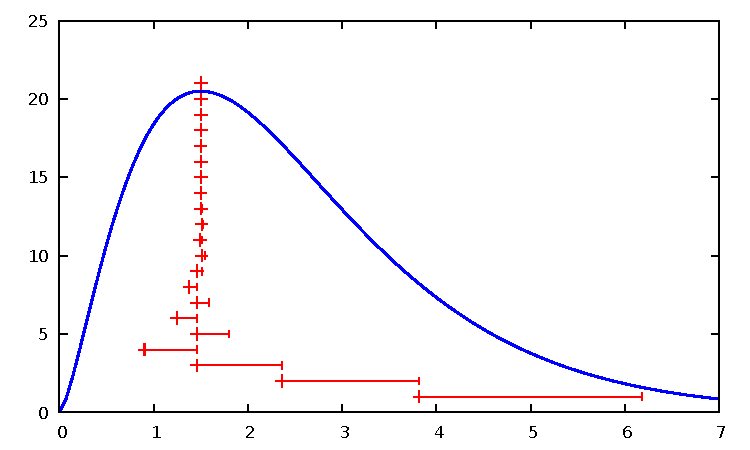
\includegraphics[scale=0.8]{figures/gss}
  \caption{Golden section search method: example}
  \label{fig:goldenratio}
\end{figure}


\subsection{Simulated Annealing}
\label{sec:sim-anneal}

Simulated annealing---as implemented by the gretl function
\texttt{simann}---is not a full-blown maximization method in its own
right, but can be a useful auxiliary tool in problems where
convergence depends sensitively on the initial values of the
parameters. The idea is that you supply initial values and the
simulated annealing mechanism tries to improve on them via controlled
randomization.

The \texttt{simann} function takes up to three arguments. The first
two (required) are the same as for \texttt{BFGSmax} and
\texttt{NRmax}: an initial parameter vector and a function that
computes the maximand. The optional third argument is a positive
integer giving the maximum number of iterations, $n$, which defaults
to 1024.

Starting from the specified point in the parameter space, for each of
$n$ iterations we select at random a new point within a certain radius
of the previous one and determine the value of the criterion at the
new point. If the criterion is higher we jump to the new point;
otherwise, we jump with probability $P$ (and remain at the previous
point with probability $1-P$).  As the iterations proceed, the system
gradually ``cools''---that is, the radius of the random perturbation
is reduced, as is the probability of making a jump when the criterion
fails to increase.

In the course of this procedure $n+1$ points in the parameter space
are evaluated: call them $\theta_i, i=0,\dots,n$, where $\theta_0$ is
the initial value given by the user. Let $\theta^*$ denote the
``best'' point among $\theta_1, \dots, \theta_n$ (highest criterion
value). The value written into the parameter vector on completion is
then $\theta^*$ if $\theta^*$ is better than $\theta_0$, otherwise
$\theta_n$. In other words, failing an actual improvement in the
criterion, \texttt{simann} randomizes the starting point, which may be
helpful in tricky optimization problems.

Listing~\ref{ex:simulated-annealing} shows \texttt{simann} at work as
a helper for \texttt{BFGSmax} in finding the maximum of a bimodal
function.  Unaided, \texttt{BFGSmax} requires 60 function evaluations
and 55 evaluations of the gradient, while after simulated annealing
the maximum is found with 7 function evaluations and 6 evaluations of
the gradient.\footnote{Your mileage may vary: these figures are
  somewhat compiler- and machine-dependent.}

\begin{script}[htbp]
  \scriptinfo{simulated-annealing}{BFGS with initialization via Simulated Annealing}
\begin{scode}
function scalar bimodal (matrix x, matrix A)
    scalar ret = exp(-qform((x-1)', A))
    ret += 2*exp(-qform((x+4)', A))
    return ret
end function

set seed 12334
set max_verbose on

scalar k = 2
matrix A = 0.1 * I(k)
matrix x0 = {3; -5}

x = x0
u = BFGSmax(&x, bimodal(x, A))
print x

x = x0
u = simann(&x, bimodal(x, A), 1000)
print x
u = BFGSmax(&x, bimodal(x, A))
print x
\end{scode}
\end{script}

\subsection{Nelder--Mead}
\label{sec:nelder-mead}

The Nelder--Mead derivative-free simplex maximizer (also known as the
``amoeba'' algorithm) is implemented by the function \texttt{NMmax}.
The argument list of this function is essentially the same as for
\texttt{simann}: the required arguments are an initial parameter
vector and a function-call to compute the maximand, while an optional
third argument can be used to set the maximum number of function
evaluations (default value: 2000).

This method is unlikely to produce as close an approximation to the
``true'' optimum as derivative-based methods such as BFGS and
Newton--Raphson, but it is more robust than the latter. It may succeed
in some cases where derivative-based methods fail, and it may be
useful, like \texttt{simann}, for improving the starting point for an
optimization problem so that a derivative-based method can then take
over successfully.

\texttt{NMmax} includes an internal ``convergence'' check---namely,
verification that the best value achieved for the objective function
at termination of the algorithm is at least a local optimum---but by
default it doesn't flag an error if this condition is not
satisfied. This permits a mode of usage where you set a fairly tight
budget of function evaluations (for example, 200) and just take any
improvement in the objective function that is available, without
worrying about whether an optimum has truly been reached. However, if
you want the convergence check to be enforced you can flag this by
setting a negative value for the maximum function evaluations
argument; in that case the absolute value of the argument is taken and
an error is provoked on non-convergence.

If the task for this function is actually minimization, you can either
have the function-call return the negative of the actual criterion or,
if you prefer, call \texttt{NMmax} under the alias \texttt{NMmin}.

Here is an example of use: minimization of the Powell quartic
function, which is problematic for BFGS. (The true minimum is zero,
obtained for \texttt{x} a 4-vector of zeros.)
%
\begin{code}
function scalar powell (const matrix x)
  fx1 = x[1] + 10 * x[2]
  fx2 = x[3] - x[4]
  fx3 = x[2] - 2 * x[3]
  fx4 = x[1] - x[4]
  return fx1^2 + 5.0 * fx2^2 + fx3^4 + 10.0 * fx4^4
end function

matrix x = {3, -1, 0, 1}'
printf "Initial f(X) = %g\n", powell(x)
fmin = NMmin(x, powell(x))
printf "Estimate of optimal X*:\n%14f\n", x
printf "f(X*) = %g\n", fmin
\end{code}

\section{Numerical differentiation}
\label{sec:numdiff}

\subsection{Computing a Jacobian}
\label{sec:fdjac}

Gretl offers the possibility of differentiating numerically a
user-defined function via the \texttt{fdjac} function.

This function takes two arguments: an $n \times 1$ matrix holding
initial parameter values and a function call that calculates and
returns an $m \times 1$ matrix, given the current parameter values and
any other relevant data.  On successful completion it returns an $m
\times n$ matrix holding the Jacobian.  For example,
%
\begin{code}
matrix Jac = fdjac(theta, SumOC(&theta, &X))
\end{code}
where we assume that \texttt{SumOC} is a user-defined function with
the following structure:
%
\begin{code}
function matrix SumOC (matrix *theta, matrix *X)
  matrix V = ...  # do some computation
  return V
end function
\end{code}

This may come in handy in several cases: for example, if you use
\texttt{BFGSmax} to estimate a model, you may wish to calculate a
numerical approximation to the relevant Jacobian to construct a
covariance matrix for your estimates.

Another example is the delta method: if you have a consistent
estimator of a vector of parameters $\hat{\theta}$, and a consistent
estimate of its covariance matrix $\Sigma$, you may need to compute
estimates for a nonlinear continuous transformation $\psi =
g(\theta)$. In this case, a standard result in asymptotic theory is
that
\[
\left\{
    \begin{array}{c}
      \hat{\theta} \convp \theta \\ 
      \sqrt{T} \left( \hat{\theta} - \theta \right) \convd N(0, \Sigma)
    \end{array}
\right\}
    \Longrightarrow
\left\{
    \begin{array}{c}
      \hat{\psi} = g(\hat{\theta}) \convp \psi = g(\theta) \\ 
      \sqrt{T} \left( \hat{\psi} - \psi \right) \convd N(0, J
      \Sigma J')
    \end{array}
\right\}
\]
where $T$ is the sample size and $J$ is the Jacobian
$\left.\pder{g(x)}{x}\right|_{x = \theta}$.

\begin{script}[htbp]
  \scriptinfo{delta-method}{Delta Method}
\begin{scode}
function matrix MPC(matrix *param, matrix *Y)
  beta = param[2]
  gamma = param[3]
  y = Y[1]
  return beta*gamma*y^(gamma-1)
end function

# William Greene, Econometric Analysis, 5e, Chapter 9
set echo off
set messages off
open greene5_1.gdt

# Use OLS to initialize the parameters
ols realcons 0 realdpi --quiet
a = $coeff(0)
b = $coeff(realdpi)
g = 1.0

# Run NLS with analytical derivatives
nls realcons = a + b * (realdpi^g)
  deriv a = 1
  deriv b = realdpi^g
  deriv g = b * realdpi^g * log(realdpi)
end nls

matrix Y = realdpi[2000:4]
matrix theta = $coeff
matrix V = $vcv

mpc = MPC(&theta, &Y)
matrix Jac = fdjac(theta, MPC(&theta, &Y))
Sigma = qform(Jac, V)

printf "\nmpc = %g, std.err = %g\n", mpc, sqrt(Sigma)
scalar teststat = (mpc-1)/sqrt(Sigma)
printf "\nTest for MPC = 1: %g (p-value = %g)\n", \
      teststat, pvalue(n,abs(teststat))
\end{scode}
\end{script}

Script \ref{ex:delta-method} exemplifies such a case: the example is
taken from \cite{greene03}, section 9.3.1. The slight differences
between the results reported in the original source and what
gretl returns are due to the fact that the Jacobian is computed
numerically, rather than analytically as in the book.

On the subject of numerical versus analytical derivatives, one may
wonder what difference it makes to use one method or another. Simply
put, the answer is: analytical derivatives may be painful to derive
and to translate into code, but in most cases they are much faster
than using \cmd{fdjac}; as a consequence, if you need to use
derivatives as part of an algorithm that requires iteration (such as
numerical optimization, or a Monte Carlo experiment), you'll
definitely want to use analytical derivatives.

Analytical derivatives are also, in most cases, more precise than
numerical ones, but this advantage may or may not be negligible in
practice depending on the practical details: the two fundamental
aspects to take in consideration are nonlinearity and machine precision.

As an example, consider the derivative of a highly nonlinear function
such as the matrix inverse. In order to keep the example simple, let's
focus on $2 \times 2$ matrices and define the function
\begin{code}
function matrix vecinv(matrix x)
    A = mshape(x,2,2)
    return vec(inv(A))'
end function
\end{code}
which, given $\mathrm{vec}(A)$, returns $\mathrm{vec}(A^{-1})$. As is
well known (see for example \cite{magneu88}),
\[
  \frac{\partial \mathrm{vec}(A^{-1})}{\partial \mathrm{vec}(A)} 
  = - (A^{-1})' \otimes (A^{-1}),
\]
which is rather easy to code in \app{hansl} as
\begin{code}
function matrix grad(matrix x)
    iA = inv(mshape(x,2,2))
    return -iA' ** iA
end function  
\end{code}
Using the \cmd{fdjac} function to obtain the same result is even
easier: you just invoke it like
\begin{code}
fdjac(a, "vecinv(a)")  
\end{code}

In order to see what the difference is, in terms of precision, between
analytical and numerical Jacobians, let's start from $A =
\left[\begin{array}{cc} 2 & 1 \\ 1 & 1 \end{array}\right]$. The
following code
\begin{code}
a = {2; 1; 1; 1}
ia = vecinv(a)
ag = grad(a)
ng = fdjac(a, "vecinv(a)")
dg = ag - ng
print ag ng dg  
\end{code}
gives
\begin{code}
ag (4 x 4)

  -1    1    1   -1 
   1   -2   -1    2 
   1   -1   -2    2 
  -1    2    2   -4 

ng (4 x 4)

  -1    1    1   -1 
   1   -2   -1    2 
   1   -1   -2    2 
  -1    2    2   -4 

dg (4 x 4)

 -3.3530e-08  -3.7251e-08  -3.7251e-08  -3.7255e-08 
  2.6079e-08   5.2150e-08   3.7251e-08   6.7060e-08 
  2.6079e-08   3.7251e-08   5.2150e-08   6.7060e-08 
 -2.2354e-08  -5.9600e-08  -5.9600e-08  -1.4902e-07 
\end{code}
in which the analytically-computed derivative and its numerical
approximation are essentially the same. If, however, you set $A =
\left[\begin{array}{cc} 1.0001 & 1 \\ 1 & 1 \end{array}\right]$ you
end up evaluating the function at a point in which the function itself
is considerably more nonlinear since the matrix is much closer to
being singular. As a consequence, the numerical approximation becomes
much less satisfactory:
\begin{code}
ag (4 x 4)

 -1.0000e+08   1.0000e+08   1.0000e+08  -1.0000e+08 
  1.0000e+08  -1.0001e+08  -1.0000e+08   1.0001e+08 
  1.0000e+08  -1.0000e+08  -1.0001e+08   1.0001e+08 
 -1.0000e+08   1.0001e+08   1.0001e+08  -1.0002e+08 

ng (4 x 4)

 -9.9985e+07   1.0001e+08   1.0001e+08  -9.9985e+07 
  9.9985e+07  -1.0002e+08  -1.0001e+08   9.9995e+07 
  9.9985e+07  -1.0001e+08  -1.0002e+08   9.9995e+07 
 -9.9985e+07   1.0002e+08   1.0002e+08  -1.0001e+08 

dg (4 x 4)

     -14899.      -14901.      -14901.      -14900. 
      14899.       14903.       14901.       14902. 
      14899.       14901.       14903.       14902. 
     -14899.      -14903.      -14903.      -14903. 
\end{code}
Moreover, machine precision may have its impact: if you take $A =
0.00001 \times \left[\begin{array}{cc} 2 & 1\\ 1 &
    1 \end{array}\right]$, the matrix itself is not singular at
all, but the order of magnitude of its elements is close enough to
machine precision to provoke problems:
\begin{code}
ag (4 x 4)

 -1.0000e+10   1.0000e+10   1.0000e+10  -1.0000e+10 
  1.0000e+10  -2.0000e+10  -1.0000e+10   2.0000e+10 
  1.0000e+10  -1.0000e+10  -2.0000e+10   2.0000e+10 
 -1.0000e+10   2.0000e+10   2.0000e+10  -4.0000e+10 

ng (4 x 4)

 -1.0000e+10   1.0000e+10   1.0000e+10  -1.0000e+10 
  1.0000e+10  -2.0000e+10  -1.0000e+10   2.0000e+10 
  1.0000e+10  -1.0000e+10  -2.0000e+10   2.0000e+10 
 -1.0000e+10   2.0000e+10   2.0000e+10  -4.0000e+10 

dg (4 x 4)

     -488.30      -390.60      -390.60      -195.33 
      634.79       781.21       390.60       585.98 
      634.79       488.26       683.55       585.98 
     -781.27      -976.52      -781.21      -1367.3 
\end{code}

\subsection{Computing a Hessian}
\label{sec:Hessian}

In principle, you can use the \cmd{fdjac} function repeatedly to
evaluate higher-order derivatives. However, you should be aware that
you may encounter rather serious numerical issues. For this reason,
gretl provides a function, similar to \cmd{fdjac}, for computing
a Hessian directly, called \cmd{numhess}.

An example follows:
\begin{code}
function scalar quad(matrix x, matrix A )
    return 0.5*qform(x', A)
end function

function matrix coljac(matrix x, matrix A)
    return fdjac(x, quad(x, A))'
end function

A = {23, -11; -11, 118}
x = {1;1}

set fdjac_quality 2
H0 = fdjac(x, "coljac(x, A)")
H1 = numhess(x, "quad(x, A)")
printf "\n%14.8f", H0
printf "\n%14.8f", H1
\end{code}
In this example, we use the function \texttt{quad} for evaluating a
simple quadratic form $f(x) = \frac{1}{2} x'Ax$, for which the Hessian
is trivially the matrix $A$. The matrix \texttt{H0} is obtained by
using \cmd{fdjac} twice (at its best quality, that is with Richardson
extrapolation on); the matrix \texttt{H1}, instead, is obtained
directly via the \cmd{numhess} function. The result of the above
script is:
\begin{code}
   22.99788411  -10.99983724
  -10.99902343  117.99161784

   23.00000000  -11.00000000
  -11.00000000  118.00000000
\end{code}
which makes it apparent how much better the second result is (note
that \texttt{H0} is not even symmetric, as it should be). 

\section{Numerical integration}
\label{sec:numint}

The main tool that gretl offers in this area is integration via
Gaussian quadrature. In practice, the evaluation of an integral of the
kind
\begin{equation}
  \label{eq:quadint}
  C = \int_{A} f(x) \omega(x) \mathrm{d}x
\end{equation}
is approximated via a suitable linear combination of the form
\begin{equation}
  \label{eq:quadsum}
  C \simeq \sum_{i=1}^q f(x_i) w(x_i) ,
\end{equation}
where the $q$ ``quadrature points'' $x_1, x_2, \ldots, x_q$ are
suitably chosen and the corresponding weights $w(x_i)$ ensure that the
approximation is optimal.

The \cmd{quadtable} function provides quadrature points and weights
for the following list of problems:
\begin{center}
\begin{tabular}{ccp{0.4\textwidth}}
  \hline
  \textbf{Integral} & \textbf{Technique} & \textbf{Note}\\
  \hline
  $\int_{-\infty}^{\infty} f(x) e^{-x^2} \mathrm{d}x$ &
  Gauss--Hermite & see below for the relationship with the Gaussian distribution\\
  $\int_{0}^{\infty} f(x) e^{-x} \mathrm{d}x$ &
  Gauss--Laguerre & can be used for evaluating Laplace transforms numerically \\
  $\int_{a}^{b} f(x) \mathrm{d}x$ &
  Gauss--Legendre & by default, $a=-1$ and $b=1$ \\
  \hline
\end{tabular}
\end{center}
The \cmd{quadtable} function returns a $q \times 2$ matrix with the
$x_i$ points in the first column and the corresponding weights $w_i$
in the second, so in practice you compute the desired integral of
$f(x)$ by applying that function to the first column and then
computing the inner product of the result by the second column.

In econometrics, Gaussian quadrature is most commonly used for
evaluating expectations of functions of Gaussian random variables,
that is, integrals of the form
\[
  E\left[f(X)\right] = \int_{-\infty}^{\infty} f(x) \varphi(x)
  \mathrm{d} x
\]
In this case, Gauss--Hermite quadrature can be readily applied,
provided one modifies the integral above via a suitable change of
variable, namely by defining $z = x/\sqrt{2}$ so that
\[
  \int_{-\infty}^{\infty} f(x) \frac{1}{\sqrt{2 \pi}} e^{-x^2/2}
  \mathrm{d} x =
  \frac{1}{\sqrt{\pi}} \int_{-\infty}^{\infty} f(\sqrt{2} \cdot z)
  \cdot  e^{-z^2}
  \mathrm{d} z
\]
For example, consider the following script, in which we evaluate
$E(e^X)$ and $E[\cos(X)]$ via Gaussian quadrature.
\begin{code}
q = 10
Q = quadtable(q)

x = exp(sqrt(2) * Q[,1])
w = Q[,2] ./ sqrt($pi) 
printf "E(exp(x)) = %16.14f (exact = %16.14f)\n", x'w, exp(0.5)

x = cos(sqrt(2) * Q[,1])
w = Q[,2] ./ sqrt($pi) 
printf "E(cos(x)) = %16.14f (exact = %16.14f)\n", x'w, exp(-0.5)
\end{code}
The result is
\begin{code}
E(exp(x)) = 1.64872127069823 (exact = 1.64872127070013)
E(cos(x)) = 0.60653065971146 (exact = 0.60653065971263)
\end{code}
Higher values of $q$ will give a more precise approximation.

In fact, the full form of \cmd{quadtable}---which supports three
optional arguments besides the required
$q$---provides a shortcut which saves you the hassle of having to
recalculate the integral with the change of variable. Suppose you want
something like
\[
  C = E\left[f(X)\right] \qquad \mathrm \qquad X \sim N(\mu, \sigma^2)
\]
Then you can use the syntax \cmd{quadtable(q, 1, m, s)}, where the 1
indicates Gauss--Hermite integration and the two final arguments give
the mean and standard deviation. So for example if you want to compute
$E(X^2)$, where $X \sim N(1, 0.25)$, you could use
\begin{code}
# Note: no rescaling needed
Q = quadtable(q, 1, 1, 0.5)
printf "E(X^2) = %6.4f (exact = %6.4f)\n", (Q[,1].^2)'Q[,2], 1.25
\end{code}
which yields
\begin{code}
  E(X^2) = 1.2500 (exact = 1.2500)
\end{code}
See the \GCR\ for more details.

%%% Local Variables: 
%%% mode: latex
%%% TeX-master: "gretl-guide"
%%% End: 
